\chapter{\fancyname{NodeMPST}: Back-End Session Type Web Development}
\label{chap:node}

In this chapter we present \fancyname{NodeMPST},
our session type API generation strategy for 
server-side endpoints implemented on the Node.js runtime \cite{node}.
We continue to use the running example of the \tprotocol{Adder}
protocol, and refer to the FSM of the \trole{Svr} endpoint
(\cref{fig:addersvrfsm}) throughout this chapter.

\begin{figure}[!b]
\centering
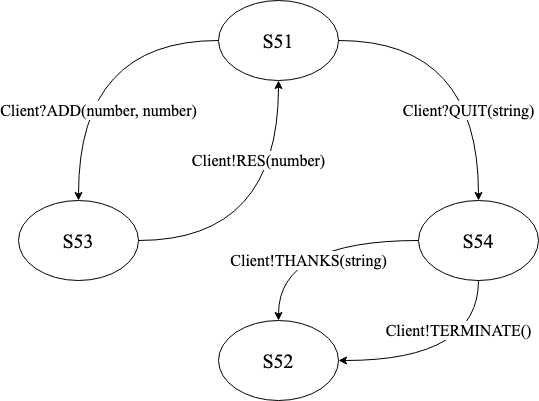
\includegraphics[width=0.5\textwidth]{AdderSvrFSM}
\captionof{figure}{\trole{Svr} Endpoint FSM
in \tprotocol{Adder} protocol}
\label{fig:addersvrfsm}
\end{figure}

\section{Challenges}
\label{section:nodechallenges}
\begin{itemize}
\item session type implementation on the node runtime
\item need to provide consistency under the single-threaded event loop model
\item provide idiomatic event-driven APIs
\item provide static guarantees where possible -- communication mismatch and channel linearity
\item typescript's type system is gradual, structural and non-linear -- session type api generation examples that provide static guarantees on channel usage build upon target language type system's support for linear resources
\end{itemize}

As outlined in \cref{section:typescript}, TypeScript's type system
is neither affine nor linear, so we need to work around the 
limitations of the language to enforce linear usage of channel resources.
Similarly, we need to 
the language does not provide
built-in constructs for enforcing linear channel usage.

\section{Approach}
\label{section:nodeapproach}

We motivate our approach from \cite{PureScript2019, HuJava}
to generate \textbf{handler-style APIs} to be implemented
by developers.
This aligns with idiomatic TypeScript practices of defining
\textit{callbacks} in the application logic.
We type the parameters and return values of the handlers to
reflect the message types specified in the protocol.
By strictly specifying handlers for send and receive actions,
we do not expose send and receive APIs to the developer,
making it impossible for the developer to reuse channels.

The responsibility of guaranteeing linear channel usage now falls
under the runtime that executes the EFSM.
As we generate this for the developer,
we can provide \textbf{static}
linearity guarantees by construction.

\begin{itemize}

\item inspired by purescript approach -- hide the channel resource so they are linear by construction, simply expose callbacks and handlers
\item the runtime executes the EFSM, performs the send and receive actions through the websocket, and invokes the correct handler as required
\item provide overview of the files we generate (and forward reference in the correct subsections) -- EFSM, Runtime, `others' (exclude cancellation)
\end{itemize}

When executing \fancyname{SessionTS} to generate code for the
\trole{Svr} endpoint specifying the \texttt{node} target,
the developer obtains the following files:

\begin{itemize}
\item \textbf{EFSM.ts:} TypeScript types constructed for 
the EFSM encoding (\cref{section:nodeefsm});
\item \textbf{Svr.ts:} Session runtime for executing the EFSM 
(\cref{section:noderuntime}).
\end{itemize}

\section{EFSM Encoding}
\label{section:nodeefsm}

In addition to states and transitions, we generate 
TypeScript constructs
for relevant metadata in the state machine: this includes
\textit{roles}, \textit{labels} and \textit{message structures}.


The EFSM contains more than just states and transitions

The generated \textbf{EFSM.ts} file encodes all information
available 

\begin{figure}
\begin{lstlisting}[language=javascript,tabsize=2]
export namespace Roles {...};
export namespace Labels {...};
export namespace Message {...};

export namespace Handler {...};

abstract class ISend {...};
abstract class IReceive {...};
abstract class ITerminal {...};
export namespace Implementation {...};

export type EfsmTransitionHandler =
	(implementation: Implementation.Type) => void;
export type MessageHandler = (message: any) => void;
\end{lstlisting}
\captionof{lstlisting}{Structure of generated EFSM.ts file 
for server endpoints}
\label{lst:nodeefsmfile}
\end{figure}

\begin{itemize}
\item callbacks -- type aliases for each state (handler)
\item need a way for the runtime to distinguish between states (implementation)
\item attempt at using conditional types, but because they handle conditional union types in a distributed way (give example), cannot be statically typed
\item alternative -- use discriminated union by wrapping in an Implementation class
\item all non-terminal states will `return' the successor implementation -- very difficult to resolve in the type-checker in the runtime (give example of what it may look like) -- solve by giving each state implementation the `advance' function to respect the event-driven nature of everything, so they can call it on completion
\item visualise the interaction between runtime and states as a sequence diagram for message passing
\end{itemize}

\begin{figure}[!ht]
\begin{lstlisting}[language=javascript, tabsize=2]
// Inside the Message namespace...
export type S54THANKS = {
	label: Labels.S54.THANKS,
	payload: [string],
};
export type S54TERMINATE = {
	label: Labels.S54.TERMINATE,
	payload: [],
};

export type S54 = | S54THANKS | S54TERMINATE;
\end{lstlisting}
%\label{}
\captionof{lstlisting}{Generated Message Type Definition for State 54}
\end{figure}

\subsection{Handler APIs}

We collect the APIs that the developer needs to implement
under the \texttt{Handler} namespace. 
As a design choice, we \textit{do not} generate handlers for
terminal states, because the semantics of inactivity mean
there is nothing to handle.
We outline how the generated API differs between sending
and receiving states.

\paragraph{Send}
We generalise deterministic send actions as a trivial \textit{selection}, 
as motivated from the theory (\dots).

\begin{figure}[!ht]
\begin{lstlisting}[language=javascript, tabsize=2]
// Inside the Handler namespace...
export type S54 = 
	| [Labels.S54.THANKS, Message.S54THANKS['payload'],
		Implementation.S52] 
	| [Labels.S54.TERMINATE, Message.S54TERMINATE['payload'], 
		Implementation.S52];
\end{lstlisting}
\captionof{lstlisting}{Generated Type for \trole{Svr} Send State
in \tprotocol{Adder} protocol}
\end{figure}

\paragraph{Receive}
\begin{itemize}
\item very short -- go over the structure and give examples
\item show how it extends for polyadic payloads
\end{itemize}

\begin{figure}[!ht]
\begin{lstlisting}[language=javascript,tabsize=2]
// Inside the Handler namespace...
export type S51 = {
	[Labels.S51.ADD]: (...payload: Message.S51ADD['payload']) =>
		Implementation.S53,
	[Labels.S51.QUIT]: (...payload: Message.S51QUIT['payload']) => 
		Implementation.S54,
}
\end{lstlisting}
\captionof{lstlisting}{Generated Type for \trole{Svr} Receive State
in \tprotocol{Adder} protocol}
\end{figure}

As with send states,
we generalise deterministic receive actions as a trivial \textit{branch}, 
as motivated from the theory (\dots).

\subsection{Terminal}
\begin{itemize}
\item basically nothing here -- can highlight the provided type alias to provide a better developer experience
\end{itemize}

\section{Runtime}
\label{section:noderuntime}

\begin{itemize}
\item public API -- provide seam for websocket server and implementation
\item private API -- carry out the session
\end{itemize}

\subsection{Managing Connections}
\begin{itemize}
\item use set and partial object to keep track of pending connections
\item ws event listeners
\item forward reference that we need to manage cancellations here too
\end{itemize}

\subsection{Executing the EFSM}
\begin{itemize}
\item implementation details delegated to the actual implementation states
\item constructor binds all methods (that will be passed to other components0 to `this' because of how javascript works with respect to the scoping of `this' (give short example -- or ignore, if this is in the background for typescript)
\item advance -- use discriminated union to figure out what to pass to the state (send -- sendMessage, receive -- register)
\end{itemize}

\begin{figure}[!ht]
\centering
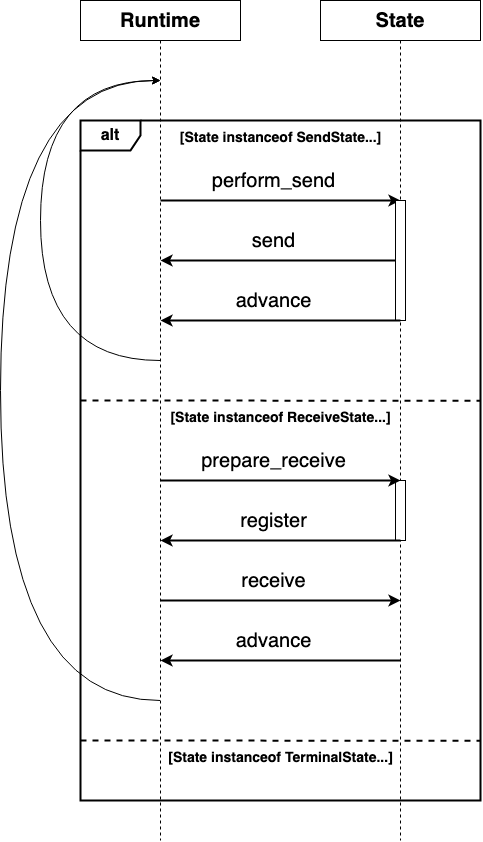
\includegraphics[width=0.5\textwidth]{NodeRuntimeEFSM}
\captionof{figure}{``Message Passing'' Abstraction of EFSM Execution for
Server Endpoints}
\label{fig:noderuntimeefsm}
\end{figure}

\subsection{Handling Message Sends}
\begin{itemize}
\item very short (just for completeness in the report) -- messages are serialised JS objects (in JSON notation) sent and decoded on the other end, type-correct by construction
\end{itemize}

\subsection{Handling Message Receives}
\begin{itemize}
\item motivate the edge case that message can arrive in the websocket (in succession) before the handler is registered
\item motivate the edge case that message can arrive `out of protocol order' 
\item explain the double queue system and how that provides consistency -- emphasising that this works because of the single-threaded typescript runtime
\end{itemize}

\begin{figure}[!ht]
\centering
\begin{subfigure}[b]{0.8\textwidth}
\centering
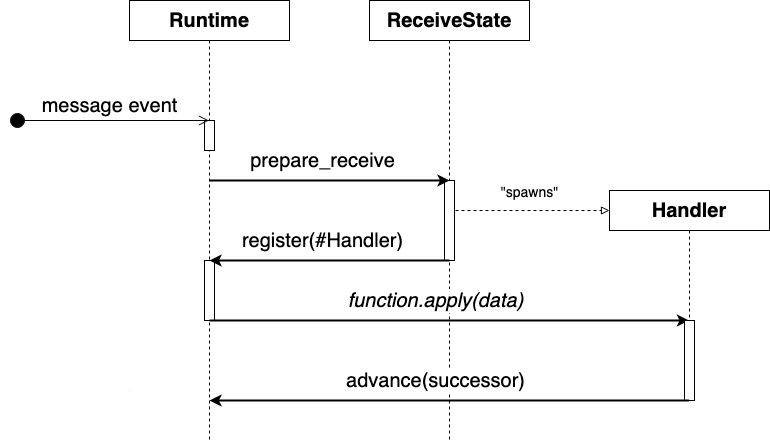
\includegraphics[width=\textwidth]{NodeRuntimeReceive2}
\caption{Message processed before transitioning to receive state}
\label{subfig:nodereceivemsgfirst}
\end{subfigure}
\hfill
\begin{subfigure}[b]{0.8\textwidth}
\centering
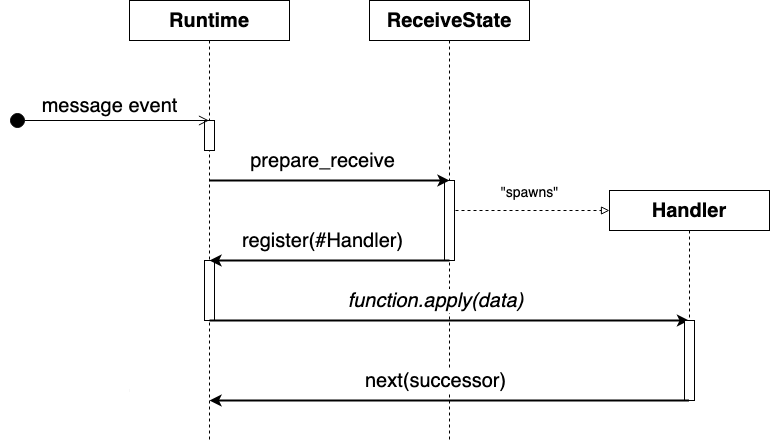
\includegraphics[width=\textwidth]{NodeRuntimeReceive1}
\caption{Message processed after transitioning to receive state}
\label{subfig:nodereceivehandlefirst}
\end{subfigure}
\captionof{figure}{Possible Orderings for Handling Message Event and Preparing
Receive State}
\label{fig:nodereceivecompare}
\end{figure}

\subsection{Handling Termination}
\begin{itemize}
\item design choice that the client is the one that closes the connection because of the centralised role of the server
\item forward reference that this gives opportunity to extend support for general protocols, as in those protocols, the server's terminal state doesn't imply it's terminal for everyone else
\end{itemize}

\section{Alternative Designs}
\label{section:nodealt}

The main alternative EFSM encoding would be similar to those
presented in \cite{Hybrid2016}, which encodes
each EFSM state as a separate class and expose communication APIs
(e.g. send and/or receive) that respect the permitted transitions at
that state. 

\begin{lstlisting}[language=scribble]
global protocol OneAdder(role Client, role Svr) {
	NUM1(number) from Client to Svr;
	NUM2(number) from Client to Svr;
	SUM(number)  from Svr to Client;
}
\end{lstlisting}

\begin{figure}[!h]
\centering
\begin{subfigure}{\textwidth}
\begin{lstlisting}[language=javascript, tabsize=2]
const logic = async (init) => {
	const [x, num2] = await init.receive();
 	const [y, sum] = await num2.receive();
	return sum.send(x + y);
}
\end{lstlisting}
\caption{\dots}
%\label{...}
\end{subfigure}
\hfill
\begin{subfigure}{\textwidth}
\begin{lstlisting}[language=javascript]
const logic = new S4({
	NUM1: (x) => new S6({
		NUM2: (y) => ([Labels.S7.SUM, [x + y], new S5()]),
	}),
});
\end{lstlisting}
\caption{\dots}
%\label{...}
\end{subfigure}
\captionof{figure}{\dots}
%\label{...}
\end{figure}

\begin{itemize}
\item exposing channel resources like the java example -- less idiomatic (not-event-driven), need runtime linearity checks like the java example
\item `hardcoded' switch case runtime like the TSOP papers -- doesn't best leverage the type system
\end{itemize}

\section{Limitations}
\label{section:nodelimitations}

\begin{itemize}
\item verbose
\item state identifiers are in the API
\item performance aspect with class-based handlers
\end{itemize}


\section{Summary}
\begin{itemize}
\item static guarantees on channel linearity and communication mismatch (up to the use of `any)
\item handling receives introduce consistency problems, but we deal with it properly here
\end{itemize}